\chapter{The Reduction}
% Covers: outline C0-C4: the slip; bisection realized; the mediant walk; the surd; descent
% Chapter language (per Ch1 protocol): the descent Topology -> Algebra -> Geometry.
% Begins in algebra; ends drawn. Figures from S2 onward (the arrow's geometry end).

\section{One earn-site, three readings}
% Node-map: C0 (THE PROXIMITY SLIP -- named in full on first use and kept, per the
% turn-517 precision requirement; slip(d) = 18/d^2, measured at unit distance,
% slip(1) = 18; the ONE earn-site of the eighteen; fan-out to coupling / radius /
% crossing-with-the-five; first sight of where the bracket lives, between d=1 and d=2).
% C0 CARRIED status plain. NO figure (S2's tree owns the first drawing).
% Gate: turn 517 (Ch4 S1, ~850 words).

The last chapter ended with three counts declared safe to spend --- eighteen, five,
eighteen --- and this chapter spends them. It is the descent: it begins in algebra,
and by its end the argument will be drawing pictures, because that is where its arrow
points. But the first thing owed is an origin story. A reader who has been told that
every number names its earn-site is entitled to ask: where, exactly, does eighteen
come from?

It comes from one measurement, and the measurement has a full name that this book will
keep: the proximity slip. The name is kept deliberately, because a different quantity
with "slip" in its casual name --- a second difference, with a chapter of its own ---
appears later in this argument, and the two share a word and nothing else. Where
confusion is possible, this one is always the proximity slip; the reader is asked to
hold the distinction, because the argument's own working notes once briefly confused
the two sites, and the discipline of full names is what unwound it.

Here is the measurement. Set the measuring text at its natural station and displace it
--- move the description a distance $d$ away, in the machine's own units of
distinguishability. The elaboration slips: the count changes, and the change is
systematic. Displace a little and the slip is large; displace further and it falls
away with the square of the distance:

\begin{center}
$\mathrm{slip}(d) \;=\; \dfrac{18}{d^{\,2}}.$
\end{center}

At unit displacement, $\mathrm{slip}(1) = 18$ --- and that eighteen is not a fitted
parameter but a measured ratio of counts, of exactly the immune shape the last chapter
proved: a numerator over the bulk of the run, the bulk cancelling, eighteen exactly.
This is the one earn-site. The number is measured here, at unit displacement of the
proximity slip, once --- and nowhere else in the argument is an eighteen measured, so
every eighteen the reader meets from now on is this one, spent again.

It is spent three ways, and the fan-out deserves to be seen whole. The coupling of the
last chapter --- the first of the three immune inputs --- is this eighteen: the
numerator that survives the mass product is the proximity slip at unit distance. The
radius --- the third input --- returns the same measured value at its own station: the
natural unit of orbit, where the instrument reads eighteen again, the one measurement
answering at a second post. And the crossing --- the subject of the rest of this
chapter --- is where the eighteen meets the five. One earn-site, three readings: it is
the argument's strongest single economy, and the reader should weigh it both ways. As
a strength: there is one honest source, and everything downstream declares its
dependence on it --- no scattered constants, no second bookkeeping. As an exposure:
break the one site and all three readings break together. The argument accepts that
exposure with its eyes open, because each of the three spendings carries its own
immunity theorem from the last chapter --- the concentration is in the earning, not in
the safety --- and because a single named source is exactly what makes the falsifiers
of the final chapters short enough to state.

Now the five, and its origin is the section's last and best lesson in economy. The
five is not an independent measurement, and the book says so proudly, because the
record does. It is the eighteen again, read through the proximity slip at the second
post: at $d = 2$ the slip reads $18/4$, four and a half; the instrument's arithmetic
keeps the floor of that reading, four; and the target is one past the floor --- five.
The same real-input cancellation as everything else makes this structural: the bulk
divides out, so four-plus-one is a fact about the ratio, not about any run's mood. The
fan-out is therefore total. Not two spendings plus an independent target, but one
measured root and three structural transforms: the coupling is the slip at the first
post; the target is one past the slip's floor at the second post; the radius is the
same value at the orbit's post. One root, three paths. The exposure statement sharpens
accordingly, and without false comfort: break the one site and everything breaks. And
Chapter 3's three theorems stand exactly as stated --- each transform carries its own
immunity; what was never asserted there, and is withdrawn here, is independence.

Watch, then, what happens as the displacement grows. At $d = 1$ the proximity slip
reads eighteen, far above. At $d = 2$ it reads four and a half --- already below the
five that its own floor at that post determines. Somewhere between one and two units
of displacement, the falling slip crosses the five: a seam the instrument cut with its
own knife, one section before the knife is named. That crossing is the event the whole
measurement is built to locate. The reader has just
seen, in one line of arithmetic, where the bracket of Chapter 1 lives: between $d = 1$
and $d = 2$, in the machine's own units, there is a displacement at which slip equals
target, and the number that displacement determines is the one the book has promised
to bracket. Everything from here to the readings chapter is the discipline of trapping
it honestly.

Trapping it requires a way of cutting the interval between one and two --- and not an
imported way. The machine must cut with its own knife or the earn-site discipline dies
on the spot. It turns out the machine has a knife: its own act of reduction, the
rewriting it was born doing, cuts intervals in a manner as old as arithmetic --- and
when the cuts are drawn, they make a tree. That is the next section, and it is where
this chapter starts drawing.

\section{The walk that cuts}
% Node-map: C1 (the machine's reduction REALIZED AS interval-cutting -- the division
% walk, remainder-and-swap; "realized as" per C1's PARTIAL, the identity never claimed),
% C2 (the mediant as the cut; the walk's tree = the device's topology). THE BOOK'S FIRST
% FIGURE: the Stern-Brocot tree's first levels, walk's path toward the crossing marked.
% Ledger rows in-prose: Euclid (division walk), Farey (mediant), Stern & Brocot (tree).
% Fencepost stop PROMISED for S3 (ledger 10). Gate: turn 518 (Ch4 S2, ~1000 words).

The machine's knife was promised, and here it is. It is not a new attachment bolted on
for the occasion; it is the machine's native act, the one it performs all day: given a
ratio of counts, reduce it. Divide, keep the remainder, swap, and divide again --- how
many whole fives in eighteen, remainder three; how many threes in five, remainder two;
and so on downward until a remainder runs out. This is the division walk, and it is
the oldest algorithm on record: Euclid wrote it down twenty-three centuries ago as the
way to find what two numbers have in common, and the ledger credits him for it. The
machine did not learn it from Euclid. Remainder-and-swap is simply what reduction is,
and a machine built to rewrite ratios walks it as naturally as water runs downhill.

One discipline before the walk is put to work, because the book owes the reader its
usual exactness. This book does not claim that the machine's rewriting is the division
walk in some deep and final identity --- that identity is a research question, and the
book does not owe it. What the book shows is machinery: when the machine reduces the
ratios this measurement produces, its steps realize the division walk --- the same
cuts, in the same order, stopping at the same places. Realized as, not revealed to be.
Everything the argument needs is in the realization, and nothing in the identity.

Now watch the walk cut intervals rather than numbers, because that is the use the
crossing requires. The tool is the mediant. Take two fractions standing as fences
around a stretch of the line, $a/b$ on the left and $c/d$ on the right. Their mediant
is the fraction a child would invent by adding tops and bottoms:

\begin{center}
$\dfrac{a}{b} \;<\; \dfrac{a+c}{b+d} \;<\; \dfrac{c}{d}$
\end{center}

and the child would be right, because the mediant always lands strictly between its
parents. It is, moreover, the cheapest interior point there is: no fraction with a
smaller denominator lands in the gap. The reader should hear Chapter 2 in that
sentence --- the cheapest sufficient name is the honest one --- and hear it as more
than an echo. The mediant is the cheapest-decision discipline arrived in arithmetic:
each cut of an interval is the least decision that separates, and the walk that makes
such cuts inherits, cut by cut, the ground's own economy. The study of which fractions
sit cheapest in which gaps is Farey's, and his ledger row is earned here.

Begin, then, with the crudest fences imaginable around everything --- zero on the
left, the infinite on the right --- and cut by mediants, always keeping the two fences
that still bracket what is sought. The cuts, drawn, make a tree: every cut a node,
its two child regions the two ways the walk can turn next. The first levels are worth
seeing whole, with the walk toward this argument's crossing marked:

\begin{figure}[htbp]
\centering
\begin{tikzpicture}[level distance=1.35cm,
  level 1/.style={sibling distance=5.2cm},
  level 2/.style={sibling distance=2.7cm},
  level 3/.style={sibling distance=1.5cm},
  every node/.style={font=\small}]
\node (root) {$\frac{1}{1}$}
  child[gray] {node {$\frac{1}{2}$}
    child[gray] {node {$\frac{1}{3}$}}
    child[gray] {node {$\frac{2}{3}$}}
  }
  child {node {$\frac{2}{1}$}
    child {node {$\frac{3}{2}$}
      child[gray] {node {$\frac{4}{3}$}}
      child {node (walkend) {$\frac{5}{3}$}}
    }
    child[gray] {node {$\frac{3}{1}$}
      child[gray] {node {$\frac{5}{2}$}}
      child[gray] {node {$\frac{4}{1}$}}
    }
  };
\node[below=0.3cm of walkend, font=\small\itshape] {the walk continues toward the crossing};
\end{tikzpicture}
\caption{The first levels of the tree the cuts make. Every positive fraction appears
exactly once, already in lowest terms. The marked path is this measurement's walk:
the crossing of Section 1 lies between $1$ and $2$, so the walk enters at $\frac{1}{1}$,
turns toward $\frac{2}{1}$, and begins cutting --- $\frac{3}{2}$, then $\frac{5}{3}$,
each mediant the cheapest cut of the fences then standing.}
\end{figure}

This tree has a name and two discoverers --- a mathematician and a clockmaker, Stern
and Brocot, who found it independently, the clockmaker because gear trains are ratios
and he needed the cheapest gears that would do --- and their ledger row is earned by
the figure. Two of its properties pay the argument's bills. Every positive fraction
appears in the tree exactly once, already in lowest terms: the tree is a complete
roster of the ratios, with no duplicates to audit away. And the path to any fraction
is unique: to know where the walk went is to know everything about how it got there,
so a walk's transcript --- like every transcript in this book --- is a text whose
parse settles all questions.

The crossing of the first section lies between one and two, and the reader can now
watch the first cuts land. The fences begin at $1$ and $2$. The first mediant cuts at
$\frac{3}{2}$; the crossing sits above it, so the left fence advances and the walk
turns toward $\frac{5}{3}$; above again, and again the fence advances. The walk is
closing in, from below, in runs of same-direction turns --- and the length of each
straight run, the number of turns before the walk next changes direction, is a number
with a standing in arithmetic all its own: a partial quotient, a count in the walk's
own currency. Those runs are what the argument counts. How many of them the walk is
permitted --- where the counting is made to stop --- is governed by the fencepost of
Chapter 2, and the showing of that stop, run by run to the fence and not one run
past it, is the next section's whole business.

\section{The count to the fencepost}
% Node-map: C3 (the surd named: the crossing = sqrt(18/5), computable inside the counts
% via the earned integer square root; STITCH CLAUSE at the naming per turn 519 -- both
% numbers under the root trace to the one earn-site), the STOP shown (ledger entry 10
% DISCHARGED: three runs to the fencepost of Ch2, not one run past), the bracket pinned
% AS THE WALK'S OUTPUT (the reading itself is Ch5 D1's -- handoff stated), C4 landed
% here as runs-as-descent with "realized as" held (BFGS quartet + Newton row).
% Euler/Lagrange row (convergents as best approximations). SECOND FIGURE: the interval
% closing in three runs. Gate: turn 519 (Ch4 S3, ~1000 words, chapter closer).

The crossing can now be given its name. The event the walk hunts is the displacement
at which the falling slip meets the five, and the algebra is one line: eighteen over
$d^2$ equals five where $d^2$ equals eighteen fifths, so

\begin{center}
$d \;=\; \sqrt{\dfrac{18}{5}}\,,$
\end{center}

the square root of eighteen over five --- and the reader should pause on what stands
beneath that root. Both numbers trace to the single earn-site of this chapter's first
section: the eighteen is the proximity slip at the first post, and the five is one
past the slip's floor at the second. The surd is not a formula with two inputs; it is
one measurement quarreling with itself at two distances, and the crossing is where the
quarrel settles. A square root, moreover, is no threat to the earn-site discipline:
the argument computes it inside the counts, by the earned integer square root --- the
whole-number part of the root of a count is itself found by counting, no continuum
required --- so the surd never leaves the machine's own arithmetic.

Now the walk is run at last, and the reader may watch each run land. The quarry is
irrational --- no fraction ever equals it, the walk can run forever --- which is
precisely why what matters is not where the walk ends but where it is made to stop.
The first run overshoots: from its entry the walk steps up and plants a fence above
the crossing. The second run answers: one step down, a fence below. The third run
climbs: from below, fence by fence, each mediant the cheapest cut of the interval
then standing, the lower fence advancing on the crossing without ever reaching it.
And there the walk stops.

It stops for neither of the reasons a numerical procedure usually stops. Not fatigue:
the machine would run a fourth run as cheerfully as the third. Not precision achieved:
the quarry is irrational and no run achieves it. It stops because the count of runs
has reached the fencepost. Three runs is the count --- and the reader has known since
Chapter 2 exactly which three that is: the read-off length of the side-by-side
roster, the limit the ground can point to but not touch. The walk is permitted its
three runs because three is what the ground earned, and it is refused a fourth
because past the fencepost there is nothing generated to stand on. Chapter 2's
sentence was written as grammar; here it becomes operational, and the promise the
last two chapters made --- that the reader would watch the deepening procedure run
its count to the fencepost and stop there --- is discharged in the watching.

The stop has an ancient adversary, and this is the place to meet him. Zeno observed
that a runner who must first cover half the remaining distance, then half of what
remains of that, has infinitely many stretches to cross and so --- the dichotomy ---
never arrives. The walk's quarry is exactly of Zeno's kind: the crossing is
irrational, every run leaves a remainder, and a walk resolved to arrive would run
forever. The device's answer is not to run the race faster but to decline its terms.
It never enters the regress, because the regress lives on infinite divisibility and
the walk is discrete, its count finite and earned. Three runs, then the cut --- and
where Zeno's runner is forever short of a point, the walk stands holding an
interval: the point refused, the neighborhood kept.

What the stopped walk leaves standing is two fences with the crossing pinned between
them, and that interval is the walk's whole output:

\begin{figure}[htbp]
\centering
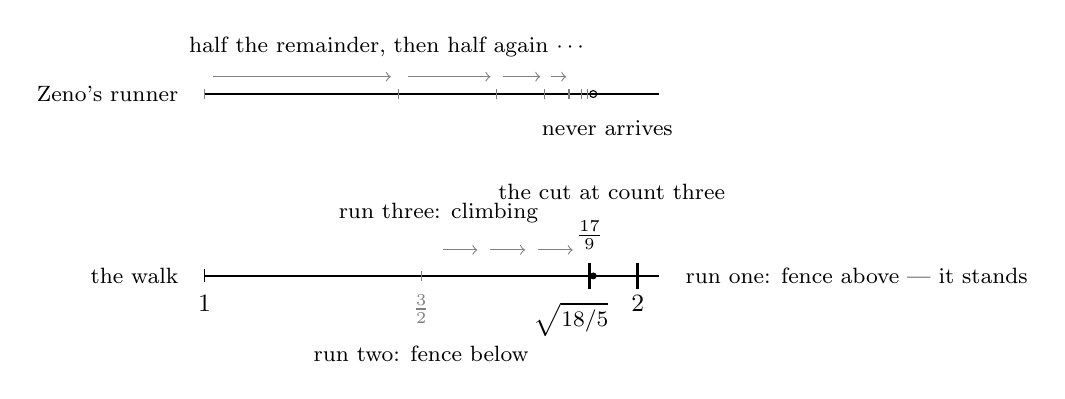
\begin{tikzpicture}[scale=5.5, every node/.style={font=\small}]
% Beat one: Zeno's dichotomy — the halvings that never arrive
\draw[thick] (1,0.42) -- (2.05,0.42);
\node[left=6pt] at (1,0.42) {\footnotesize Zeno's runner};
\foreach \x in {1, 1.4487, 1.6731, 1.7853, 1.8414, 1.8694, 1.8834}
  \draw[gray] (\x,0.408) -- (\x,0.432);
\draw[->, gray] (1.02,0.46) -- (1.43,0.46);
\draw[->, gray] (1.47,0.46) -- (1.66,0.46);
\draw[->, gray] (1.69,0.46) -- (1.775,0.46);
\draw[->, gray] (1.80,0.46) -- (1.835,0.46);
\node[above=10pt] at (1.42,0.42) {\footnotesize half the remainder, then half again $\cdots$};
\draw (1.8974,0.42) circle (0.008);
\node[below=6pt] at (1.93,0.42) {\footnotesize never arrives};
% Beat two: the walk — three runs, then the cut
\draw[thick] (1,0) -- (2.05,0);
\node[left=6pt] at (1,0) {\footnotesize the walk};
\foreach \x/\l in {1/{$1$}, 2/{$2$}} \draw (\x,-0.015) -- (\x,0.015) node[below=6pt] {\l};
\draw[gray] (1.5,-0.012) -- (1.5,0.012) node[below=5pt, gray] {$\frac{3}{2}$};
\node[right=6pt] at (2.05,0) {\footnotesize run one: fence above --- it stands};
\node[below=22pt] at (1.5,0) {\footnotesize run two: fence below};
\draw[->, gray] (1.55,0.06) -- (1.63,0.06);
\draw[->, gray] (1.66,0.06) -- (1.74,0.06);
\draw[->, gray] (1.77,0.06) -- (1.85,0.06);
\node[above=8pt] at (1.54,0.05) {\footnotesize run three: climbing};
\fill (1.8974,0) circle (0.008);
\node[below=6pt, xshift=-8pt] at (1.8974,0) {\footnotesize $\sqrt{18/5}$};
\draw[very thick] (1.8889,0.03) -- (1.8889,-0.03);
\node[above=6pt] at (1.8889,0) {\footnotesize $\frac{17}{9}$};
\draw[very thick] (2,0.03) -- (2,-0.03);
\node[above=24pt] at (1.94,0) {\footnotesize the cut at count three};
\end{tikzpicture}
\caption{Zeno's dichotomy, and the device's answer to it. Above, the runner who must
halve the remaining distance forever: the crossing is irrational, so arrival is an
infinite errand and the runner is always short of it. Below, the same quarry hunted
on the device's terms: three runs --- above, below, climbing --- then the cut at the
fencepost, leaving two standing fences with $\sqrt{18/5}$ pinned between them. The
escape is not a faster chase but a refused one: the regress needs infinite
divisibility, and the walk, discrete and finite, stops at the earned count and keeps
the interval instead of the point. Carried into the reading's units --- a translation
the next chapter performs --- the fences are the $129.6$ and $137.7$ of Chapter 1:
the bracket, earned as the walk's whole output.}
\end{figure}

Two credits are owed on this interval, and the ledger takes both. The fences the walk
leaves are not merely close; each is the best approximation of its size --- no
fraction with so small a denominator lies nearer the crossing --- and that
distinction, best-of-its-cost, belongs to the tradition of continued fractions, the
long study of exactly these stopped walks, with Euler and Lagrange at its head. And
the walk's runs admit a second reading the ledger also credits: each run uses the
standing fences --- where they sit and how the crossing fell between them --- to
choose its next advance, which is the shape of a descent that steers by accumulated
curvature rather than by a map of the whole terrain: a quasi-Newton descent, in the
tradition of Newton and of the four authors of its modern form. Here the book's
discipline holds as it did for the division walk: the runs are realized as such a
descent --- same fences, same advances, same stop --- and nothing hangs on whether
they secretly are one.

The chapter's work is done, and the handoff is exact. The walk has produced an
interval: two fences, three runs deep, with the square root of eighteen over five
pinned between them. What that interval asserts --- the reading, its value in the
book's units, its falsifier, and the difference between the bracket the argument
stands behind and the deeper value it merely displays --- is the next chapter's
property, and the next chapter is the one the whole book has been walking toward:
the readings.
